\documentclass{article}
\usepackage[utf8]{inputenc}
\usepackage[T1]{fontenc}
\usepackage[utf8]{inputenc}
\usepackage{amsmath}
\usepackage{tikz,pgfplots}
\usepackage{tikz-network}
\usetikzlibrary{shapes,decorations,arrows,calc,arrows.meta,fit,positioning}
\usepackage{color, colortbl}

\begin{document}

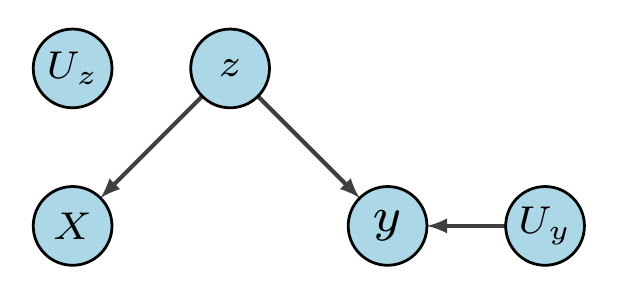
\begin{tikzpicture}
\Vertex[x=1,size = 1,label = $X$, fontscale = 2]{X}
\Vertex[size =1, x=5,label = $y$, fontscale =2.5]{Y}
\Vertex[size=1,x=3,y=2,fontscale = 2,label = $z$]{Z}
\Vertex[size=1,x=7,y=0,label = $U_y$,fontscale = 2]{Uy}
\Vertex[size=1,x=1,y=2,label = $U_z$,fontscale = 2]{Uz}
\Edge[Direct](Uy)(Y)
\Edge[Direct](Z)(X)
\Edge[Direct](Z)(Y)
\end{tikzpicture}

\end{document}